\documentclass[10pt,journal,compsoc]{IEEEtran}

\usepackage{cite}
% correct bad hyphenation here
\hyphenation{op-tical net-works semi-conduc-tor}
\usepackage[utf8]{inputenc} %para introdução de caracteres especiais
\usepackage[english]{babel}
\usepackage{tikz}
\usepackage{scalefnt}
\usepackage{comment} 
\usepackage{graphicx}
\usepackage{url}

\begin{document}

\title{Wall Following STDR}
\author{\^{A}ngela Cardoso~and~In\^{e}s Caldas%
\thanks{Faculdade de Engenharia da Universidade do Porto, Rua Dr. Roberto Frias, 4200-465 Porto, Portugal.}}

\IEEEtitleabstractindextext{%
\begin{abstract}
The developments in robotics technology motivate the need for stable and reliable autonomous robots. Using the \textit{ROS} framework and the \textit{STDR Simulator} package, a wall following robot was design and implemented. The design of the robot takes into consideration the specifications and restrictions of the problem the robot has to face, follow indefinitely a wall as soon it is discovered. A set of maps where used to test the behavior and the stability of the robot during its movement. From our tests, we observed that the robot maintained a stable movement for most of the different configurations of the maps.
\end{abstract}

% Note that keywords are not normally used for peerreview papers.
\begin{IEEEkeywords}
Mobile robots, Reactive robots, Robot sensing systems, Navigation, Robot control, Subsumption architecture
\end{IEEEkeywords}}

% make the title area
\maketitle

%%%%%%%%%%%%%%%%
% INTRODUCTION %
%%%%%%%%%%%%%%%%
\section{Introduction}
The most basic types of robotic systems are purely reactive~\cite{Reactive}. These systems do not have neither the ability to form memories, nor to use past experiences to inform current decisions. Since they are fast and rely only on the current sensor readings, instead of a map, the use of which requires very accurate localization capabilities, reactive approaches are often used for robot navigation. However, reactive navigation does not plan ahead and is therefore susceptible to local minima. 

In this project we developed a stable wall follower behavior for a simple reactive robot. The design, implementation and testing of our solution, were made with the support of the \textit{ROS} framework~\cite{ROS,AGITR} and the \textit{STDR Simulator} package~\cite{STDR}. The robot is equipped with two lasers, that allow it to sense the world around and act according to their information. 

In the following sections we will describe the architecture of our design, discuss the results and limitations of our approach and present some last remarks.

%\cite{example}

%%%%%%%%%%%%%%%%
% ARCHITECTURE %
%%%%%%%%%%%%%%%%
\section{Architecture}
\subsection{The Robot Design}

The project makes use of the \textit{ROS} framework and the \textit{STDR Simulator} package in the design of the robot and implementation of its behavior.

The robot is disk-shaped, with a radius of 0.5m and with an ideal skid steer kinematic, allowing for turns of $2\pi$ radians. It is equipped with two laser sensors to detect obstacles, each one composed of 200 rays within an angle of $\pi/4$ radians. The left sensor is $\pi/5$ radians rotated from the front of the robot and the right one is rotated $-\pi/5$ radians. The sensors have a maximum range of 3m and a minimum range of 0.1m. Additionally, the sensors are updated with a frequency of 10Hz. A schematic of the robot is presented in Figure~\ref{fig:robot}.


\begin{figure}[thpb]
\centering
\framebox{\parbox{3in}{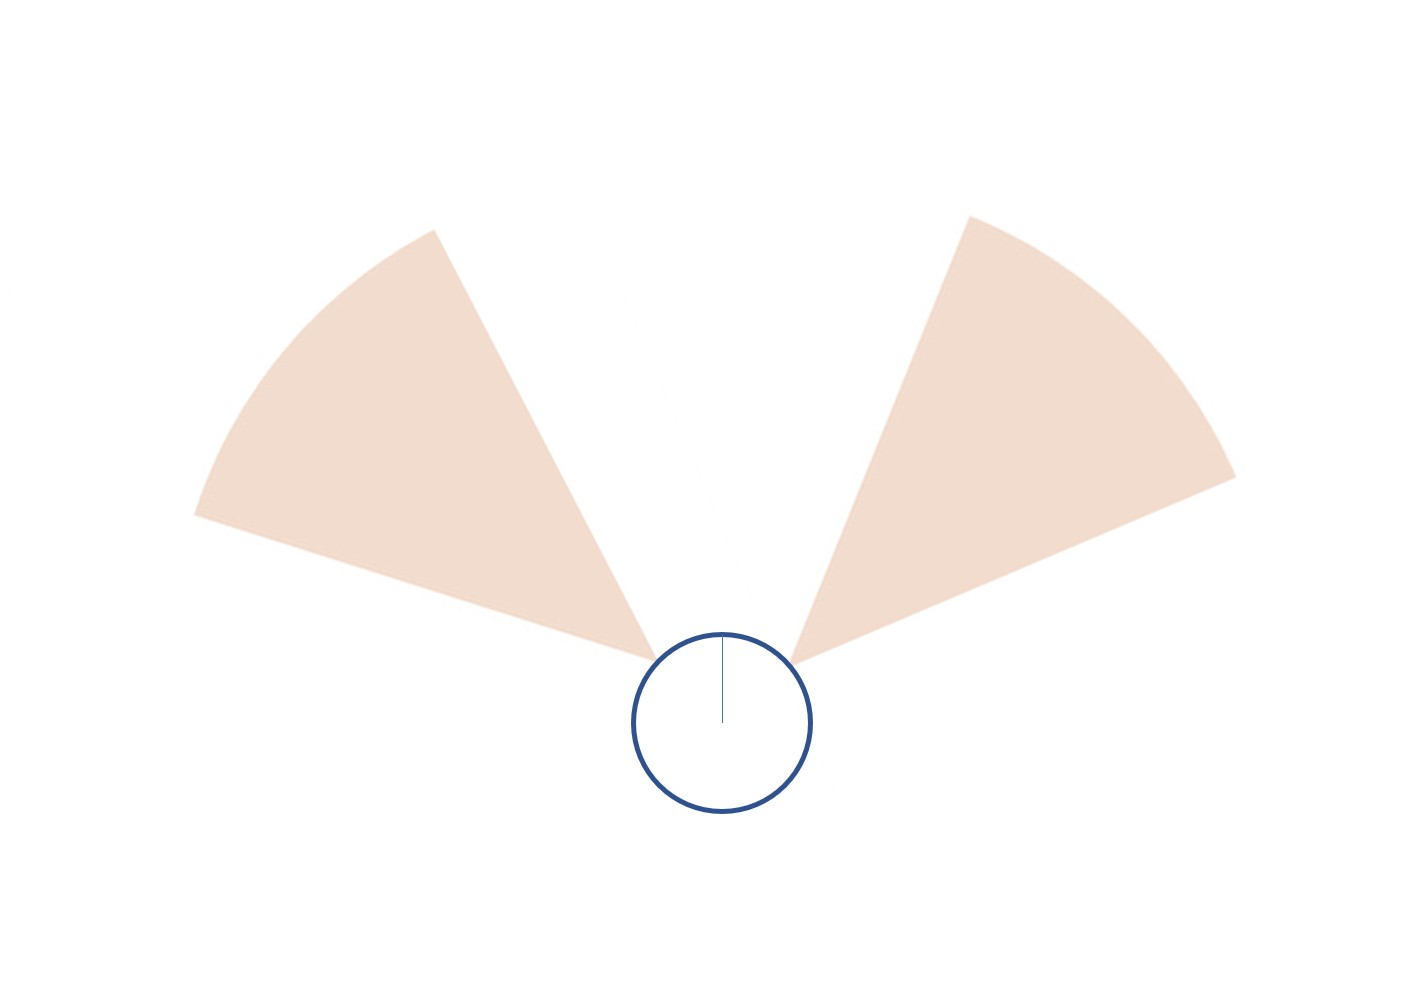
\includegraphics[scale=0.2]{img/robo.jpg}}}
\caption{Schematic of the disk-shaped robot}
\label{fig:robot}
\end{figure}


\subsection{Maps}
Three maps were developed to test the robot. They are all squares with sides of 720 pixels and a resolution of 0.05m/pixel, which entails an area of 36m$^2$ for each map. To stop the robot from trying to leave the map, all maps are equipped with a border wall.

\begin{figure}[thpb]
\centering
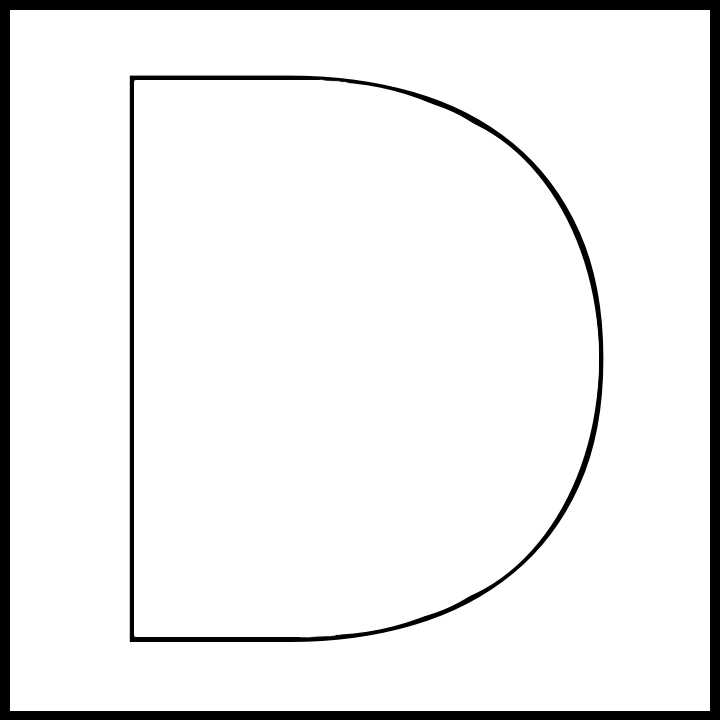
\includegraphics[scale=0.2]{img/outD.png}
\caption{The outD map}
\label{fig:outD_map}
\end{figure}

The first map we used is a large D, as shown in Figure~\ref{fig:outD_map}. The initial position of the robot is inside this large D, thus it will follow the walls from the inside. We called this map outD.

\begin{figure}[thpb]
\centering
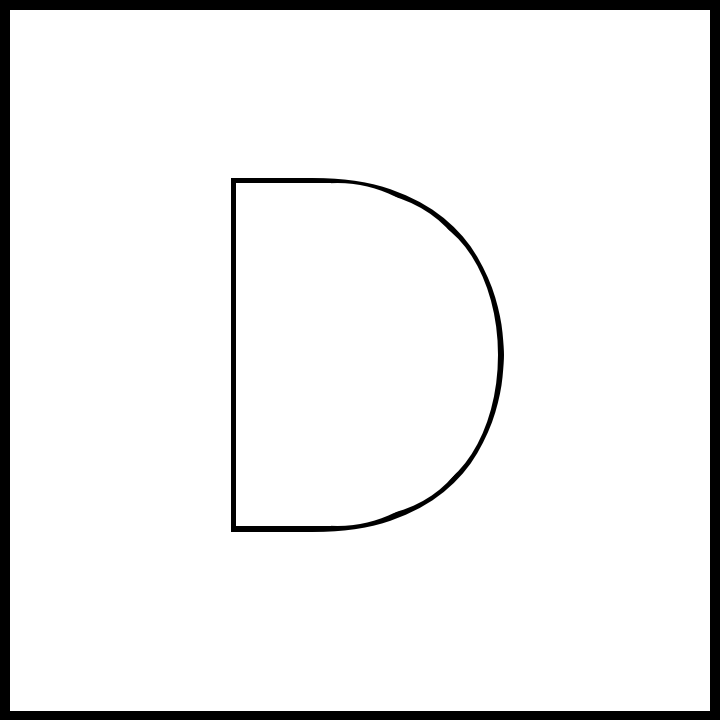
\includegraphics[scale=0.2]{img/inD.png}
\caption{The inD map}
\label{fig:inD_map}
\end{figure}

The second map is a smaller D and can be seen in Figure~\ref{fig:inD_map}. The robot is initially placed outside this D and will follow the walls from the outside. Unless it happens to find the border wall before it finds the D wall. In that case, as we will see in Subsection~\ref{subsec:map_delimiting_walls}, the robot will follow the border wall from the inside. We named this map inD.

\begin{figure}[thpb]
\centering

\includegraphics[scale=0.2]{img/DD.png}
\caption{The DD map}
\label{fig:DD_map}
\end{figure}

Finally, we used a map with a large D and a smaller D inside it, as shown in Figure~\ref{fig:DD_map}. The initial position of the robot is between both D's and it will navigate the map between both walls. We named this map DD.

\subsection{Behaviour Architecture}

The robot follows a simple subsumption based architecture.

\begin{figure}[thpb]
\centering
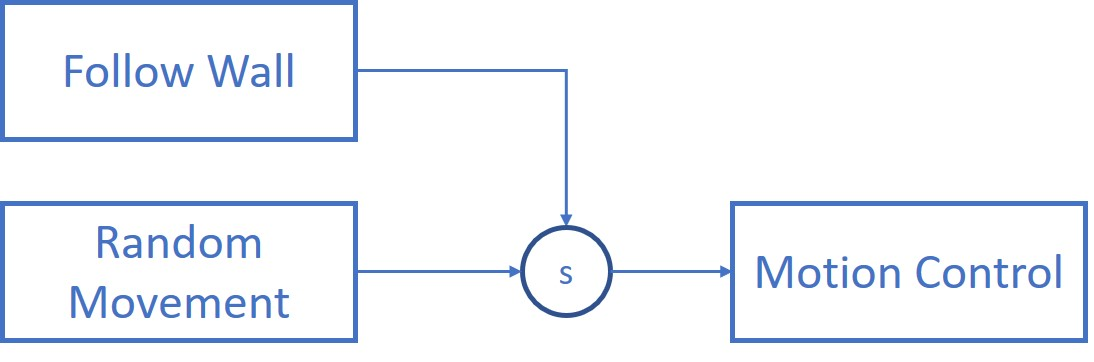
\includegraphics[scale=0.265]{img/architecture.jpg}
\caption{Subsumption architecture}
\label{fig:architecture}
\end{figure}

The architecture has two different states, as shown in the figure \ref{fig:architecture}: \textit{random movement} and \textit{follow wall}. The robot will begin with an initial movement characterized by a random linear speed $\nu$ and a random angular speed $\omega$. It will maintain this random movement up until it first discovers a wall. When it detects an obstacle, the robot will follow along its walls indefinitely. The implemented algorithms that dictate the two states are described in the following subsection. 

\subsection{Algorithms}
\subsubsection{Initial random movement}\label{subsec:initial}

Until it finds the wall, the robot moves randomly, that is, at each step it chooses random linear and angular velocities. At least this is the general idea, the actual implementation is a bit more complex. 

What happens is that in order to quickly respond to changes in the sensory data, the robot receives a new move command whenever laser data is updated. This means that previous messages are very quickly replaced with newer ones. In practice, when moving randomly the robot would move mostly forward, because turning messages would be replaced by newer messages before the robot completed the turn. Essentially, only repeated messages making the robot turn in the same direction would result in an actual turn, which is not very likely to happen.

To fix this not so random movement of the robot, we use a counter and make the robot keep turning in the same direction until the counter runs out. We still allow the magnitude of the turn and the linear velocity to change randomly, only the direction of the turn stays constant while the counter is decreasing. Each successive value of the counter is also randomized, which allows for both long and short periods of turning in the same direction.

\subsubsection{Follow wall}
Upon discovering an obstacle the goal of the robot is to follow an imaginary line at a distance $D_i$ from the wall. 

\begin{figure}[thpb]
\centering
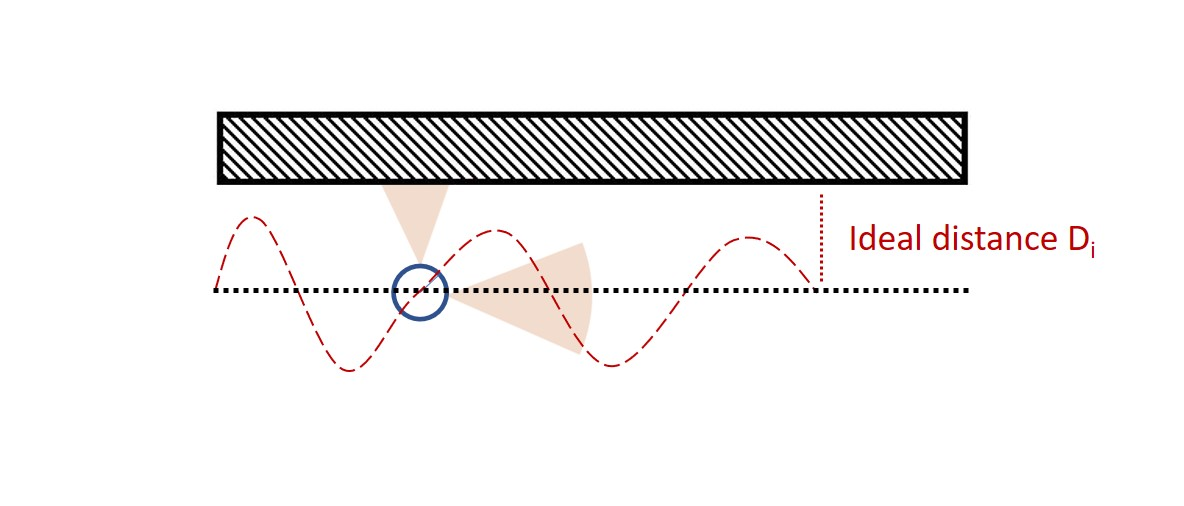
\includegraphics[scale=0.3]{img/behaviour.jpg}
\caption{Robot behaviour following a wall}
\label{fig:wall}
\end{figure}

To do so, the robot uses the readings from the lasers to correct its trajectory. Knowing from which of the sensors the measurements are coming, the robot knows if the wall is on its right or left side and can act accordingly. If the robot is getting too close to the wall (above 0.01m deviated from $D_i$), the angular velocity of absolute value $\pi/8$ is used to take it away from the all . The same happens if the robot begins to stray too far from the wall, but in the other direction. In both cases, the linear velocity of 1m/s is maintained. This behavior results in a less exaggerated version of the trajectory in figure \ref{fig:wall}.

In order to accommodate sharper turns in the wall, if the distance from the wall is 0.1m below~$D_i$, the robot will turn with an absolute value of $\pi/4$ away from the wall. It will also reduce its normal linear velocity in 90\%, that is, to 0.1m/s.

When the robot loses the readings from the laser, we know we are present in an outer corner of the map. In order to keep following the wall, the robot turns with an absolute value of $\pi/4$ in the direction of the wall, while reducing its linear velocity to 0.5m/s.

%%%%%%%%%%%
% RESULTS %
%%%%%%%%%%%
\section{Results}
For each map, the robot will be placed in a predefined position, before initiating its random movement. To validate the solution, we were interested in testing the ability of the robot to properly follow the walls present in each map and the stability of the algorithm.

The ideal distances were set to 1m for the inD and outD maps and 2m for the DD map. For all cases, an error of 0.01m from the ideal distance is allowed. The distance to the wall was measured as the robot followed the wall, resulting in the graphs shown in Figures~\ref{fig:result_outD_map},~\ref{fig:result_inD_map}~and~\ref{fig:result_DD_map}

\begin{figure}[thpb]
\centering
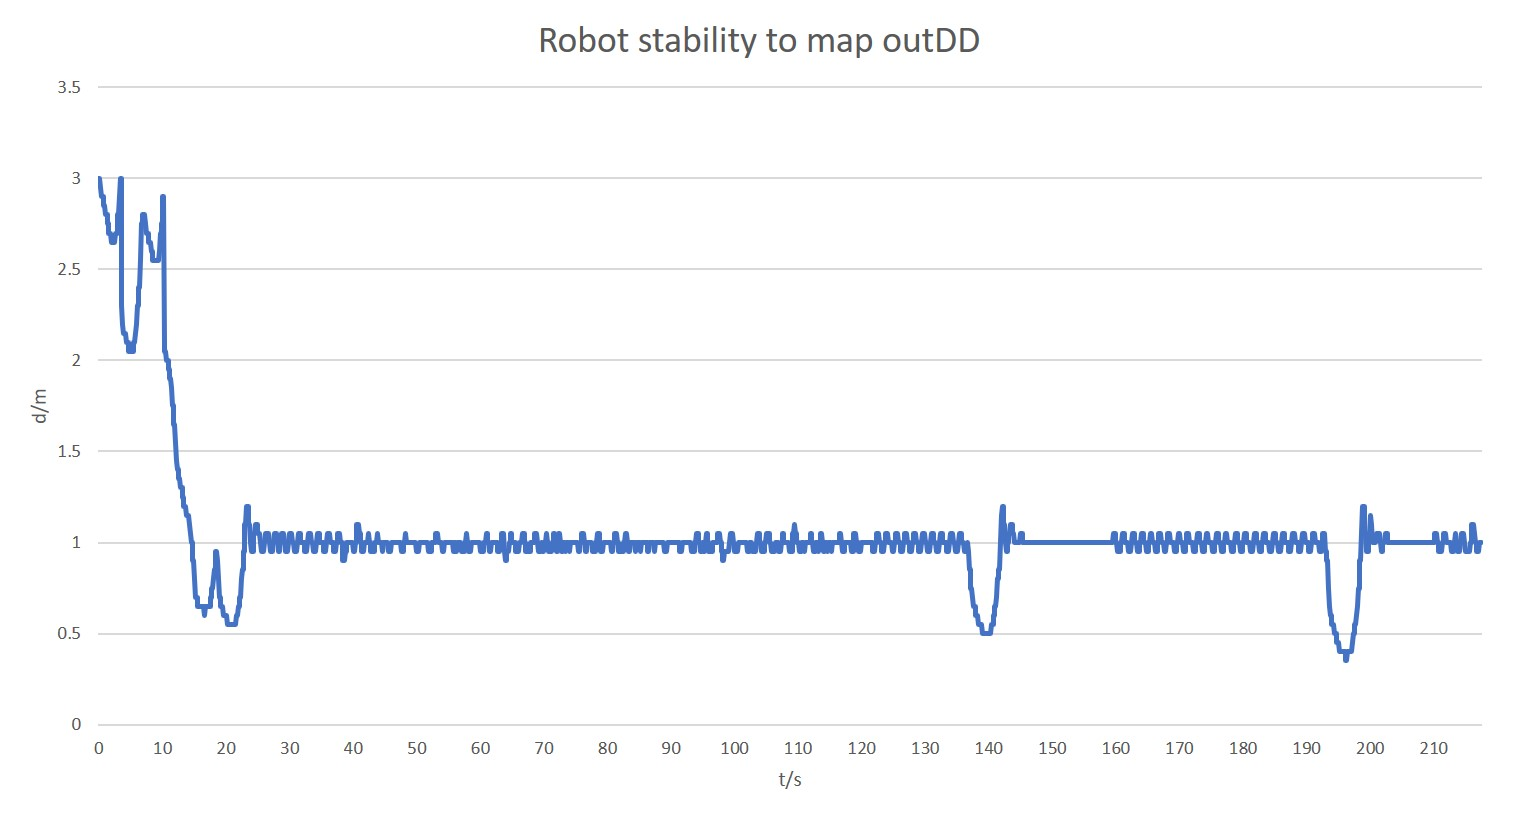
\includegraphics[scale=0.2]{img/map_outD.jpg}
\caption{Robot stability in map outD}
\label{fig:result_outD_map}
\end{figure}

For the map outD, once the robot finds the wall we can see that it keeps a stable distance around 1m from it most of the time. The exceptions seen in the graph are when the robot gets to a sharp corner of the D, then it starts getting very close to the wall and in an effort to fix this ends up going a little further away from it, finally resuming its intended distance and stable movement.

\begin{figure}[thpb]
\centering
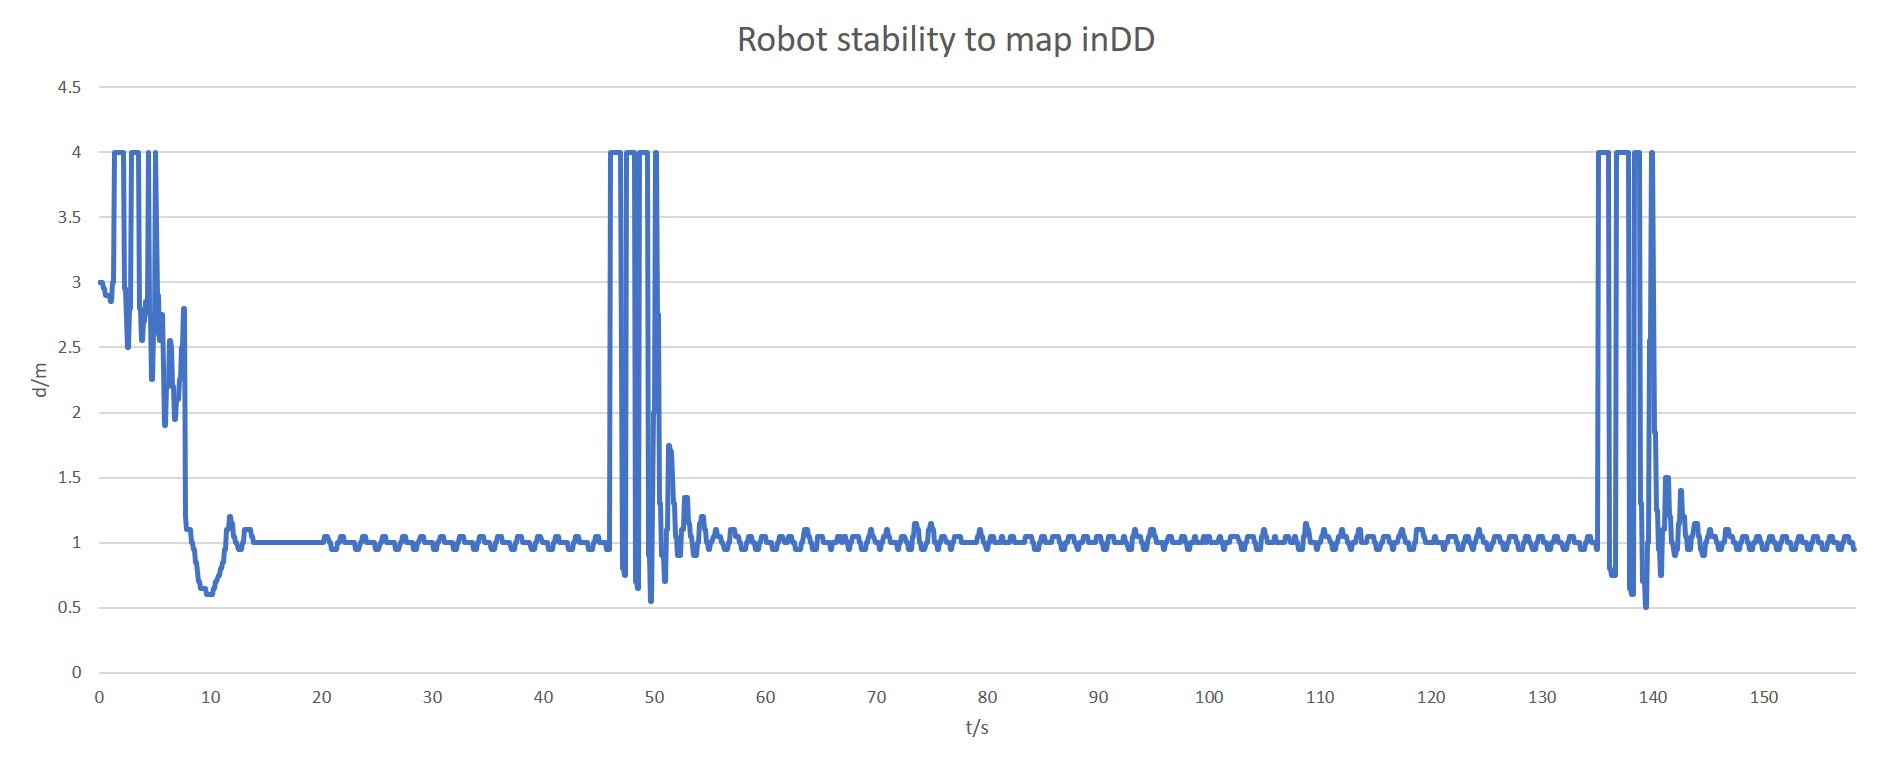
\includegraphics[scale=0.16]{img/map_inD.jpg}
\caption{Robot stability in map inD}
\label{fig:result_inD_map}
\end{figure}

As for the map inD, what happens is that in the sharp D corners, the robot temporarily looses sight of the wall, because the wall turn is away from the robot and not in front of the robot like for outD. The robot quickly turns and sees the wall again, but then needs to fix its position as it gets too close to the wall. This process is repeated a few times until the robot manages to stabilize its movements again.

\begin{figure}[thpb]
\centering
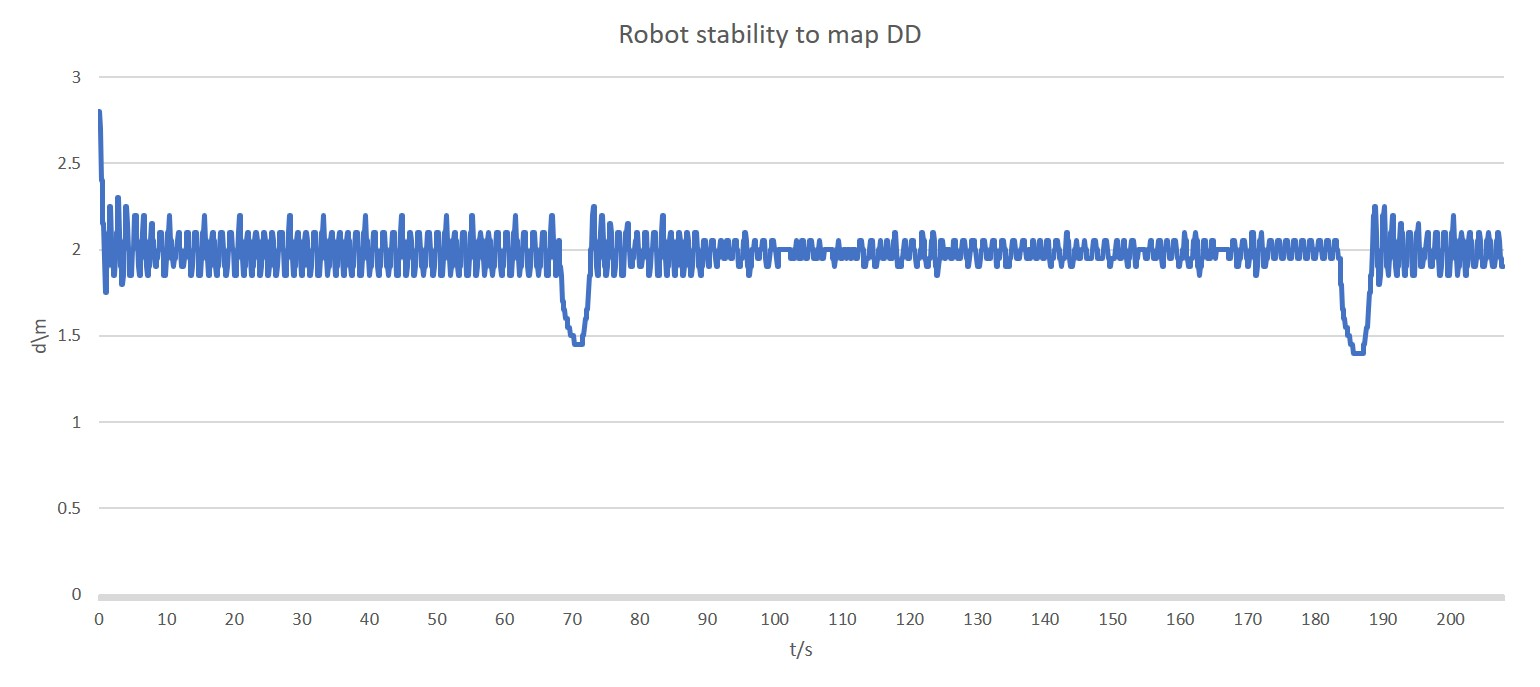
\includegraphics[scale=0.18]{img/map_DD.jpg}
\caption{Robot stability in map DD}
\label{fig:result_DD_map}
\end{figure}

The graph for the DD map is basically a repetition of the outD one. This happens because the robot chooses to follow the outside large D wall, as it is closer to it. When the robot chooses to follow the inside small D wall, the graph will be similar to that of Figure~\ref{fig:result_inD_map}.

%%%%%%%%%%%%%%%
% LIMITATIONS %
%%%%%%%%%%%%%%%
\section{Limitations}

Nothing is perfect and our wall following robot is not an exception. Most of the limitations we detected in our robot are due to the simple ideas we used to make it work. However, we still believe that the simplicity of the code is worth the restrictions it creates.

\subsection{Map delimiting walls}\label{subsec:map_delimiting_walls}

In order to keep the robot from trying to leave the map, we had to create squared walls around the map. These walls are not the ones the robot is supposed to find and follow, but if it does find these walls it will follow them forever.

Of course this only happens for the small D, whose walls the robot is supposed to follow from the outside. In the cases where the robot is inside the large D or between the two D's, it cannot move through those walls, therefore it will never find and follow the square map delimiting walls.

For the small D, we defined an initial position for the robot that is closer to the D than to the outside wall, although it sees neither of these walls. Thus, even though the initial movement of the robot will be random, it is more likely to find the small D wall and follow it. In case it finds the outside wall, the program should be stopped, but if it is not, the robot will still follow the outside wall without any problem.

\subsection{Initial random movement}

As we saw, the robot starts moving randomly until it finds a wall. Depending on the initial distance of the robot to the nearest wall and its orientation, this random search may take a long time. 

We believe this wall finding time could be improved by making it more likely for the robot to move forward than for it to turn. This is clear if the robot is inside the wall it is suppose to find, like when it is inside the large D or between both D's. But in the case where the robot is outside the small D, going forward with higher probability might increase the likelihood of the robot finding the square walls delimiting the map, before it found the D walls.

Since the map delimiting wall is only there to stop the robot from trying to leave the map and not to be followed, we kept the robot moving randomly. In any case, the only downside is longer waiting time.

\subsection{Desired wall distance}

The distance the robot tries to keep from the wall can be configured by the user. If the chosen distance is too small, the robot may not be able to turn on sharp corners. This happens because while turning the robot gets too close to the wall and perceives that it has run into it, which makes it stop altogether.

Perhaps there is some way to make the robot resume its movements if it runs into a wall, but we did not pursue that. Especially because the correct way to handle this would have been to force the robot to avoid all obstacles, which we also did not try.

As an example, for the large D that the robot follows from the inside, if the defined distance to the wall is 0.6 or less, the robot runs into the wall at the left corners of the D.

Although it was not in the initial objective, we also tested the robot in sharper corners, using a star shaped map. As we anticipated, the desired distance that the robot should keep from the wall must increase in order for it not to crash.

\subsection{Initial robot position}

If the initial position of the robot is on top or too close to a wall, it will not move. This is related to the previous limitation, as we did not try to get it to move after running into a wall. So the only way to avoid this error is to make sure that a safe initial position is configured for the robot, according to each map.

\subsection{Following two walls}

When the robot is between two walls, like when it is between the two D's, it does not follow both, that is it does not try to keep itself in the middle of both walls. We are not sure if that was the intention of the two D's assignment, but such behavior does make sense to us. The problem with trying to stay in the middle of two walls is that such behavior is different from that of trying to follow a wall at a given distance. 

There are two reasons why the robot may receive data from both lasers: either each laser detects a different wall, that is, the robot is between two walls; or both lasers detect the same wall, which may happen because the robot is facing the wall or because it is at a corner. Our way of dealing with data from both lasers is to use the laser that is closest to a wall. Unless the robot has already chosen a laser, in which case it should stick to it. This way, we avoid running into a wall because we where paying attention to the wrong laser. We also avoid turning around in an inner corner, because suddenly the other laser is closer to the wall. Plus, when the robot is facing a wall, it will eventually chose one laser, which means it will chose a direction in which to follow the wall. Unfortunately, it also means that when it is between two walls, the robot will pick the closest wall and follow it. To change this behavior, we need to be able to distinguish between the two scenarios above, and honestly we did not think further about this.

\subsection{Facing a wall}

When the robot first detects and approaches a wall, most often it will start to face that wall. Then as it goes towards the wall, because it is still further away from the wall then the desired distance, it does so in a peculiar way. Instead of going forward, it turns considerably left and right while approaching the wall.

We believe this behavior is explained by the way the robot chooses which laser to use. Suppose it chooses the left laser, then, since it is too far away from the wall, it quickly turns left, effectively making the left laser loose sight of the wall. Hence, it starts using the right laser, quickly turning right to get closer to the wall and possibly making the right laser loose sight of the wall. This may happen a few times, but eventually the robot is close enough that when turning, the chosen laser will not loose sight of the wall, leading to a normal behavior from then on.

We tried to fix this, making to robot stick to the first laser it chooses. But then it just started going around, because it had lost sight of the wall. So, although it is a strange way of going towards the wall, we kept it, because it works.

\subsection{Following a straight wall}

Sometimes, when the robot is following a straight wall, it will not go strictly forward, but very slightly deviate left and right. This is due to the noise from the lasers, and the error margin we use. We use a 0.01 error margin to quickly fix small deviations from the wall by turning $\pi/8$. If the noise is greater than 0.01, the robot will think it is too close or too far from the wall and turn a bit.

The reason for the error margin of 0.01 is because it makes the robot behave better when the wall does turn, that is, the robot follows the wall keeping a distance very close to the desired one. This happens even in sharp outer corners, that is when the robot needs to turn $\pi/2$.

\subsection{Very sharp corners}

Given the position of the lasers and their amplitude, when the robot is facing a very sharp corner, like in the outside of a star shaped wall, it may run into the corner. This happens because the robot is a little blind for small front obstacles.

However, it will only happen in a very sharp corner and if the robot is facing that corner head on.


%%%%%%%%%%%%%%%
% CONCLUSION %
%%%%%%%%%%%%%%%
\section{Conclusion}

Our implementation of a wall follower reactive robot is mostly simple, especially when it comes to the algorithm that actually makes the robot follow a wall. If the robot is getting too far from the wall it turns into the wall, if it is getting too close it turns away from the wall and otherwise it goes forward.

The end result has several limitations and at least some of them come from the simple algorithm used. For example, one could make the turn angle of the robot directly depend on how far away from the desired wall distance it is, instead of using just two rough cuts. We believe at least this idea has some merit and could be explored if the project was given some extra time.

In any case, we are pleased with our robot, because it is quite capable of stably following the proposed D map walls. Plus, with some careful distance setup it is even capable of following more complicated maps such as the star shaped ones.

\ifCLASSOPTIONcaptionsoff
\newpage
\fi

%%%%%%%%%%%%%%%%
% BIBLIOGRAPHY %
%%%%%%%%%%%%%%%%
\bibliographystyle{IEEEtran}
\bibliography{IEEEabrv,wall_bib}

\end{document}
